\chapter{Az Internet szerkezete és mérése}
%16 oldal

A következő fejezetekben az Internet struktúráját és működésének egyes aspektusait mutatom be, amelyek mélyebb megértést biztosítanak a fejlesztett mérési rendszer működésének és fontosságának megismerésében.
Az első szakaszban az internet makroszkopikus felépítését és működésének fontosabb mechanizmusait mutatom be. Ezt követően az internetes útvonalak méréseire térek ki, amely során bemutatom a mérési rendszer által használt módszerek alapjait is. Végül korábbi illetve aktívan működő Internet mérési szervezetek munkáját és projektjeit mutatom be, amely segít felmérni a mérési rendszer funkcióinak lényegét és azok fontosságát.



\section{Az internet felépítése}
%(2-3 oldal): töri, AS, BGP, nemzetközi szervezetek

%első pár saját gondolat után wikipédia cuccok
%AS kialakulások
%tipikus AS-ek, tier-ek
%http://www.tmit.bme.hu/internet


Társadalmunk fejlődésében meghatározó szerepe van, egyéb technológiai trendek mellett a szoros információs összeköttetésnek, amelyet az Internet biztosít. Történelmi tények említése nélkül az alábbiakban bemutatom a fejlődésének és működésének meghatározó részeit.

Az Internet előtt nagyobb szervezetek, egyetemek egymástól elszigetelt számítógépes há\-ló\-zat\-tal rendelkeztek. Idővel ezen szervezetek együttműködése révén a hálózataik között átjárást biztosítottak, új útvonalválasztó eljárások bevezetésével. Később ezen kezdetleges Internethez több és több saját hálózattal rendelkező csoportok, Autonóm Rendszerek\footnote{Autonomus System - AS}, csatlakoztak. Amikor már szolgáltatásként árulták erre szakosodott cégek és a gerinchálózatot is erre specializált végek bővítették,  a civil réteg számára is egyre értékesebbé és fontossá vált az Internetes elérés. Az 1990-es években robbanásszerűen terjedt el az Internetes elérés idővel majdnem minden háztartásba, az ISP\footnote{Interset Service Provider - Internet szolgáltató}-k segítségével.

Az ilyen módon organikusan növekvő Internetes hálózatban  minden résztvevő maga felel a hálózatán belüli csomagtovábbításért, és üzleti-technikai együttműködések által érik el egymáson keresztül a globális Internetet. Az üzleti megállapodások biztosítják a pénzügyi hátterét a strukturális fejlesztéseknek és a minőségi, nagy távolságokat áthidaló összeköttetések létrehozásához és üzemeltetéséhez.

A következő szakaszokban bemutatom ezen résztvevőit/alkotóit az Internetnek. Kitérek többek között az együttműködésük részleteire, valamint a rájuk ható, őket szabályozó szervezetekre.

\subsection{Erőforrások szétosztása\label{eroforrasok}}
Az Internet egyik építőköve az IP\footnote{Internet Protokoll} adatcsomag, amelyben IP cím alapján van jelölve a forrás és a cél számítógép a hálózatban. Minden kommunikáció ezen alapszik és a csomagok továbbítása ez alapján történik. Ez a cím IPv4 esetén 32, IPv6 esetén 128 biten van ábrázolva. Az összes lehetséges cím kisebb címtartományokra van osztva. Ezen felosztást mutatja be a \ref{tab:cimtartomanyok} táblázat az IPv4 esetében.

\begin{table}[ht]
	\centering
	\caption{Címtartomány kategóriák}
	\hspace{2mm}
	\begin{tabular}{ | c | c | c | r |}
	\hline
	Típus & Címtartomány & Tartalmazott címek száma & Ábrázolási példa \\ \hline

Class A & 24 bit & 16777216 db & 10.0.0.0/8\\ \hline
Class B & 20 bit & 1048576 db & 172.16.0.0/12\\ \hline
Class C & 16 bit & 65536 db & 192.168.0.0/16\\ \hline
	\end{tabular}
	\label{tab:cimtartomanyok}
\end{table}


Ezen tartományokat független nemzetközi szervezetek osztják szét az egész világon. Legfelsőbb szinten az IANA\footnote{Internet Assigned Numbers Authority - Szabad fordításban: Internetes számok felügyete} rendelkezik az egyes IP címtartományokkal. A kiosztásokat bárki szabadon megtekintheti a szervezet honlapján\footnote{\url{http://www.iana.org/assignments/ipv4-address-space/ipv4-address-space.xhtml}}.

Az IANA alá tartoznak a következő Regionális Internet Nyilvántartó szervezetek\footnote{RIR - Regional Internet Registries}: APNIC, ARIN, RIPE NCC, LACNIC, AFRINIC.
Ezen szervezetek területi felelősségeit mutatja a \ref{fig:rir-regions} ábra.

\begin{figure}[!ht]
	\centering
	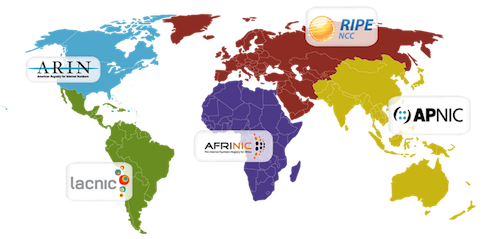
\includegraphics[width=0.9\textwidth, keepaspectratio]{figures/rir-regions.png}
	\caption{Regionális Internet Nyilvántartó szervezetek és felügyelt területeik \protect\footnotemark}
	\label{fig:rir-regions}
\end{figure}

\footnotetext{forrás: \url{https://www.apnic.net/about-APNIC/organization/history-of-apnic/history-of-the-regional-internet-registries}}

\newpage

Az egyes végfelhasználók ezen szervezeteken keresztül közvetlenül vagy közvetítéssel juthatnak saját IP címhez. Amely folyamatot részletesebben a \ref{fig:ipv4_hierarchy} ábra mutatja be, amelyen már a közvetítő szervezetek is be vannak mutatva.

\begin{figure}[!ht]
	\centering
	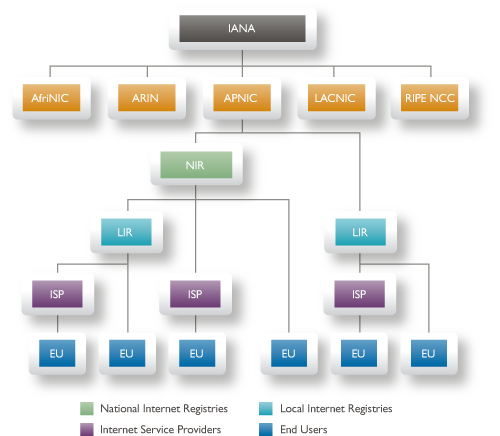
\includegraphics[width=0.7\textwidth, keepaspectratio]{figures/ipv4_hierarchy.png}
	\caption{IP tartományok kiosztásának hierarchiája\protect\footnotemark}
	\label{fig:ipv4_hierarchy}
\end{figure}

\footnotetext{forrás: \url{https://www.apnic.net/policy/ipv6-address-policy_obsolete}}


\subsection{Autonóm rendszerek}

Az egyes címtartományokkal rendelkező szervezetek, Autonóm Rendszereket alkotnak, amelyek saját hálózattal rendelkeznek. Ezen hálózatukon teljes hatalommal és felelősséggel rendelkeznek. A többi Autonóm Rendszerrel akkor lépnek kapcsolatba, amikor a címtartományukon kívüli cél felé kell elérést biztosítani vagy más Autonóm Rendszer szeretne elérést kapni az IP tartományába eső célgéphez.
Ezen forgatókönyvek esetén már nem a saját belső útvonal választási stratégiájukat használják, hanem az Autonóm Rendszerek között szabványosítottan működő protokollok alapján járnak el. Ez a BGP (Border Gateway Protocol) hálózati protokoll, amelyet minden Autonóm Rendszer külső csatlakozási pontján lévő útvonalválasztó használ. 

Ezen speciális útvonalválasztók szigorú üzleti szerződések alapján működnek, mivel az átmenő forgalom komoly pénzügyi következményekkel jár legtöbb esetben.
%Az interkontinentális csomagtovábbítás mutatja be talán a legjobban a összeköttetések létrehozásának és üzemeltetésének a költségvonzatát.
Az Autonóm Rendszerek közötti együttműködések a következő kategóriákba sorolhatóak:

\begin{itemize}
\setlength{\parskip}{0pt}
\setlength{\itemsep}{0pt plus 1pt}
  
\item \textbf{Transit} Ebben az esetben az egyik AS hozzáférést garantál a többi AS, az Internet felé.
%Egy AS lehet Single Homed, ha csak egy AS-hez csatlakozik, és lehet Multi Homed, ha több AS-en keresztül csatlakozik az Internethez.
\item \textbf{Peering} Általában hasonló nagyságú AS-ek kötnek ilyen kapcsolatot egymással, hogy kölcsönösen kicseréljék a forgalmukat, akár térítés nélkül.
\end{itemize}

Az AS-ek Interneten betöltött fő funkciója alapján pedig különböző Tier szin\-tek\-be tartozhatnak: 

\begin{itemize}
\setlength{\parskip}{0pt}
\setlength{\itemsep}{0pt plus 1pt}
  
\item \textbf{Tier\-1:} Core, azaz központi AS\-eknek is nevezik, melyek az Internet gerincét alkotják, interkontinentális összeköttetéseikkel. Egymás között megközelítőleg teljes hálót alkotva.

\item \textbf{Tier\-2:} Edge, azaz \glqq határmenti\grqq  AS-eknek is nevezik, amelyek regionálisan továbbítják az Internetes elérést. Sokszor Peering kapcsolatot kialakítva egymással.

\item \textbf{Tier\-3:} Access, azaz hozzáférési AS-eknek is nevezik, amelyek a végfelhasználóknak juttatják el az Internetes összeköttetést. Tipikusan ISP-k alkotják.
\end{itemize}

%Mennyire nehéz eldönteni melyik csoportba tartoznak pl.A határmenti AS-ek meghatározása pl homályos kicsit.



%content/eyeball/tranzit AS
%access/edge/core
%tier 3, 2, 1
%provider, customer
%transit, peering, IXP internet exchange point,
%stub AS: single homed, multihomed, 








